\chapter{Generating Normal Random Variables}

\setcounter{problem}{1}
\section{Discussion}

\begin{fullwidth}


The goal of this lab is to generate normal random variables but using the Central limit theorem instead of the inverse transform or the accept reject method. I'm not recommending this as the most efficient method, but it is a great practical application of the central limit theorem.  The hard part about all of this is using the right variance and shifting from $N(0,1)$ to the general $N(\mu, \sigma^2)$. Use filename {\tt stats/plot\_rnorm.py}.

\section{Steps}

\step First, let's define some constants $N = 100$, $TRIALS = 4000$.

\step Now, to define a function that generates normal random variables in $N(0,1)$, we rely on the fact that the sample mean, $\overline X$ from a sample $X$ of uniform distribution values, is a normal random variable.  This gives us as many normal random values as we want, one per sample $X$. We just have to tweak things so that the mean of the distribution is zero-centered and has variance 1. That shifted and scaled value is what we return from {\tt rnorm01()} that you must create in {\tt stats/stats.py}:

\begin{pyverbatim}
def rnorm01():
    "return a value from N(0,1)"
    ...
\end{pyverbatim}	

\noindent The process looks like this:

\renewcommand{\theenumi}{\Alph{enumi}}

\begin{enumerate}
\item Get $N$ uniform random values from $U(0,1)$ into $X$ using your {\tt runif()} function.
\item Then compute the mean $\overline X$.
\item Shift that value so that is zero-centered and call it $rv$.
\item We know from the CLT lab that the variance of random variable $\overline X$ is $\sigma^2 / N$, where $\sigma^2$ is the variance of the underlying distribution $U(0,1)$, but we need the variance to be 1. Scale $rv$ so that it has variance 1. Note that a ``standard normal'' variable can be created from an arbitrary normal $X$ via $Z = (X-\mu)/\sigma$. $Z$ is effectively a shifted and scaled version of the original.  Interestingly, it really just measures how many standard deviations $X$ is from $N(0,1)$.
\end{enumerate}

\step Now, let's fill in the code we need to draw a histogram and  the theoretical distribution on top using the {\tt normpdf()} from the CLT labs:

\begin{pyverbatim}
# Get X taken from TRIALS trials, plot histogram normalized to density func
X = ...
plt.axis([-4, 7, 0, 0.5]) # let's keep the same access across plot for this lab
plt.hist(X, bins=40, normed=1) # histogram should look standard normal
\end{pyverbatim}

\step Plot the real normal curve on top like we did in the CLT lab.

\step Save a PDF:

\begin{pyverbatim}
plt.savefig('rnorm01-%d-%d.pdf' % (TRIALS,N), format="pdf")
plt.show()
\end{pyverbatim}

\noindent which should look like:

\scalebox{.45}{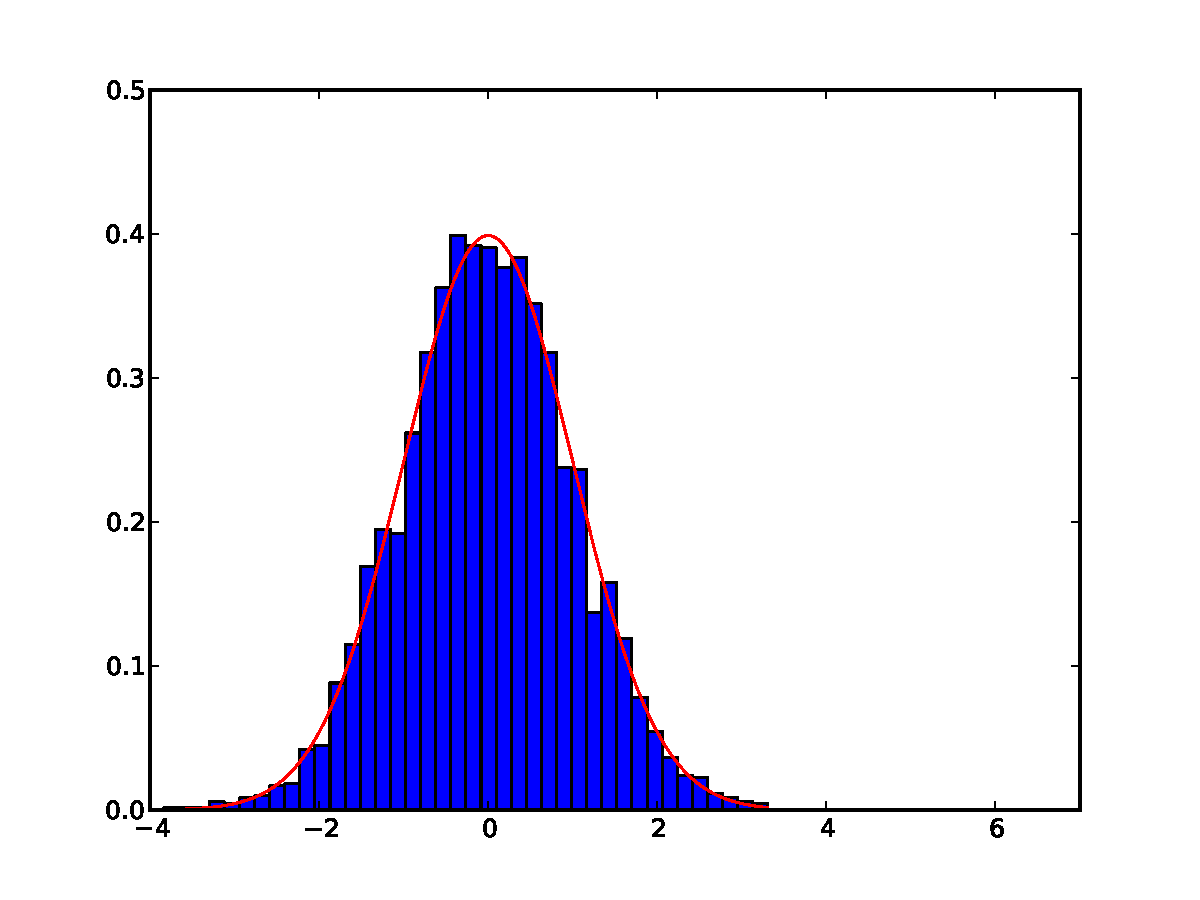
\includegraphics{figures/rnorm01-4000-100.pdf}}

\step Now define a more general method in {\tt stats/stats.py} that accepts a desired mean and variance ({\em not the mean and the standard deviation}):

\begin{pyverbatim}
def rnorm(mean, variance):
    "return a value from N(mean,variance)"
    ...
\end{pyverbatim}

\noindent We know how to get a standard normal random variable, $Z$, as we just defined {\tt rnorm01()}. To get a normal random variable with different mean and variance, we reverse the process we used to get a standard normal via $Z = (X-\mu)/\sigma$. Dust off your high school algebra and solve for $X$. That tells you how to shift and scale properly: $X = \mu+ Z\sigma$.

\step And test as before but this time use $\mu=2$ and $\sigma^2 = 2$. Save a PDF

\begin{pyverbatim}
plt.savefig('rnorm-%d-%d-%d-%d.pdf' % (MEAN,VARIANCE,TRIALS,N), format="pdf")
\end{pyverbatim}

\scalebox{.45}{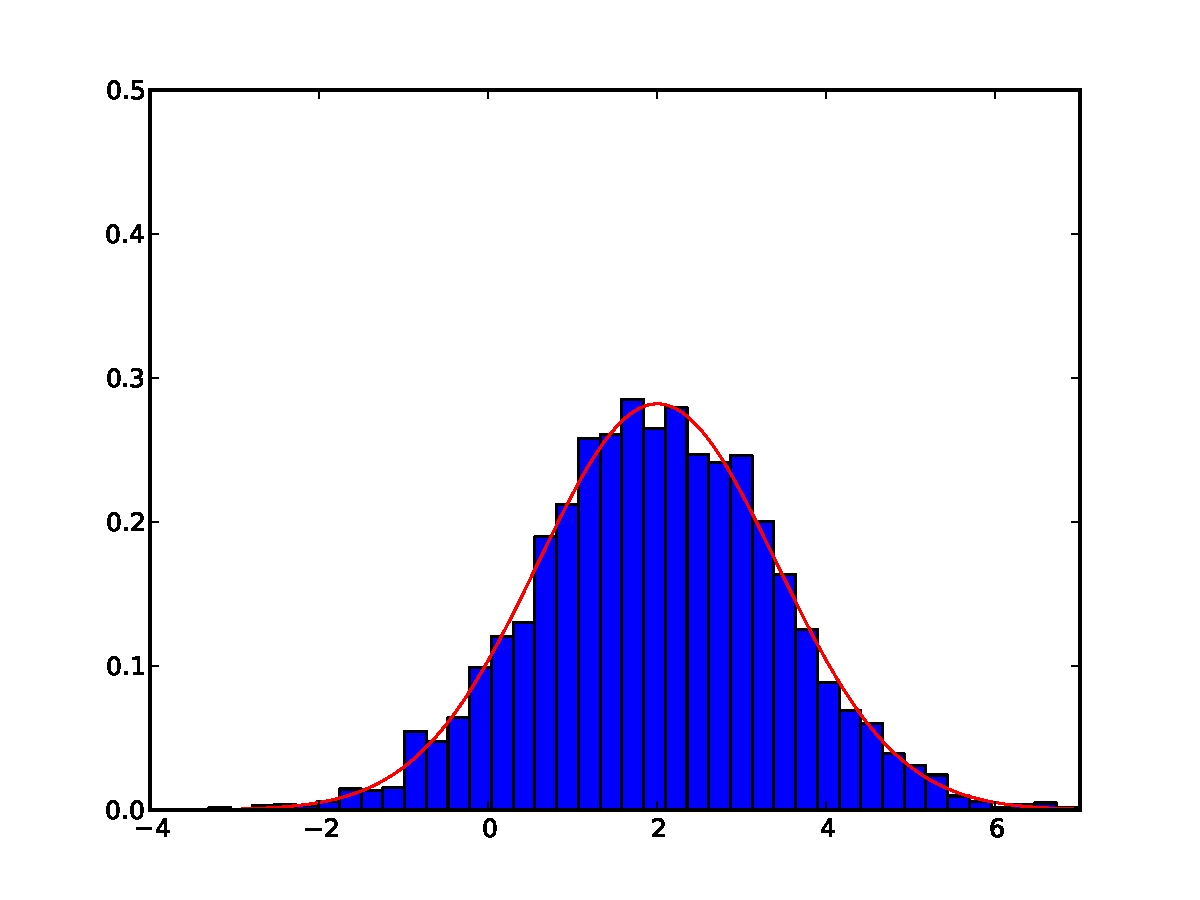
\includegraphics{figures/rnorm-2-2-4000-100.pdf}}

\begin{callout}{\bcplume}
{\bf Deliverables}. Make sure that you update {\tt stats/stats.py} and {\tt plot\_rnorm.py} is correctly committed to your repository and pushed to github. Also commit PDFs of the graphs shown above for $N(0,1)$ and $N(\mu=2,\sigma^2=2)$.
\end{callout}

\end{fullwidth}

